\documentclass{article}
\usepackage{amsmath,amsthm}
\usepackage{cancel}
\usepackage{indentfirst}
\usepackage{commath}
\usepackage{pgfplots}
\usepackage{bbold}
\begin{document}

% TODO: Pull this into a common file
% From Wikipedia, not sure where to define this yet...
\def\ci{\perp\!\!\!\perp}
\def\defeq{\buildrel\triangle\over =}
\def\E{\mathrm{E}}
\def\Var{\mathrm{Var}}
\def\Cov{\mathrm{Cov}}
\newcommand\numberthis{\stepcounter{equation}\tag{\theequation}}


\section{MLE for the Bernoulli/ binomial model}

\begin{gather}
X_i \sim Ber(\theta) \\
p(D|\theta) = \theta^{N_1}(1 - \theta)^{N_0}
\end{gather}

\begin{align*}
  \ln \left(  p(D|\theta) \right) &= \ln \left( \theta^{N_1}(1 -
                                    \theta)^{N_0} \right) \\
                                  &= \ln \left( \theta^{N-1} \right) + \ln \left( 1 - \theta
                                    \right)^{N_0} \\
                                  &= N_1 \ln \theta + N_0 \ln (1 - \theta) \\
  \od{}{\theta} \ln p(D|\theta) &= \frac{N_1}{\theta} - \frac{N_0}{1 -
                                  \theta}
\end{align*}

The log-likelihood will take a maximum when the derivative equals 0.

\begin{align*}
  0 &= \frac{N_1}{\theta} - \frac{N - N_1}{1 - \theta} \\
  0 &= N_1(1 - \theta) - \theta(N-N_1) \\
  0 &= N_1 - \theta N_1 - \theta N + \theta N_1 \\
  0 &= N_1 - \theta(N_1 + N - N_1) \\
  0 &= N_1 - \theta N \\
  \hat{\theta} &= \frac{N_1}{N}
\end{align*}
\section{Marginal likelihood for Beta-Bernoulli model}\label{3.2}
\begin{equation}\label{chain-rule-prob}
  p(X_{1:N}) = p(x_1)p(x_2|x_1)p(x_3|x_{1:2}) ... p(x_N|x_{N-1})
\end{equation}

\begin{equation}\label{bb-post-pred}
    p(X=k|D_{1:N}) = \frac{N_k + \alpha_k}{\sum_i N_i + \alpha_i}
\end{equation}

\begin{equation}\label{gamma-def}
  (\alpha - 1)! = \Gamma(\alpha)
\end{equation}

Given $D = H,T,T,H,H \defeq 1,0,0,1,1$

\begin{gather*}
  p(X=1|\alpha) = \frac{\alpha_1}{\alpha} \\
  p(X=0|\alpha, D_1) = \frac{\alpha_0}{\alpha + 1} \\
  p(X=0|\alpha, D_{1:2}) = \frac{\alpha_0 + 1}{\alpha + 2} \\
  p(X=1|\alpha, D_{1:3}) = \frac{\alpha_0 + 1}{\alpha + 3} \\
  p(X=1|\alpha, D_{1:4}) = \frac{\alpha_0 + 2}{\alpha + 4} \\
\end{gather*}

\begin{align*}
  p(D) &= p(D_{1:5}) \\
       &= p(D_1) \cdot p(D_2|D_1) \cdot p(D_3|D_{1:2}) \cdot
         p(D_4|D_{1:3}) \cdot p(D_5|D_{1:4}) \qquad \text{by ($\ref{chain-rule-prob}$)} \\
       &= \frac{\alpha_1}{\alpha} \cdot
         \frac{\alpha_0}{\alpha + 1} \cdot \frac{\alpha_0 + 1}{\alpha + 2}
         \cdot \frac{\alpha_1 + 1}{\alpha + 3} \cdot \frac{\alpha_1 +
         2}{\alpha + 4} \qquad \text{by ($\ref{bb-post-pred}$)} \\
       &= \frac{\left[ \alpha_1 (\alpha_1 + 1) (\alpha_1 + 2) \right] \left[
         \alpha_0 (\alpha_0 + 1) \right]}
         {\alpha (\alpha + 1) (\alpha + 2) (\alpha + 3) (\alpha + 4) }
  \\
       &= \frac{\left[ (\alpha_1) ... (\alpha_1 + N_1 - 1) \right] \left[
         (\alpha_0) ... (\alpha_0 + N_0 - 1) \right]}
         {(\alpha) ... (\alpha + N - 1)} \\
       &= \frac{(\alpha_1 + N_1 - 1)!}{(\alpha_1 - 1)!} \cdot
         \frac{(\alpha_0 + N_0 - 1)!}{(\alpha_0 - 1)!} \cdot
         \frac{(\alpha - 1)!}{(\alpha + N - 1)!} \\
       &= \frac{\Gamma(\alpha_1 + N_1)}{\Gamma(\alpha_1)} \cdot \frac{\Gamma(\alpha_0
         + N_0)}{\Gamma(\alpha_0)} \cdot
         \frac{\Gamma(\alpha)}{\Gamma(\alpha + N)} \\
       &= \frac{\Gamma(\alpha_1 + N_1) \; \Gamma(\alpha_0 +
         N_0)}{\Gamma(\alpha_1) \Gamma(\alpha_0)}
         \frac{\Gamma(\alpha_0 + \alpha_1)}{\Gamma(\alpha_0 + \alpha_1 +
         N)}
\end{align*}

\section{Posterior predictive for a Beta-Binomial model}

\begin{align*}
  p(x|n,D) &= Bb(x|\alpha_0', \alpha_1', n) \\
  &= \frac{B(x + \alpha_1', n-x+\alpha_0')}{B(\alpha_1',\alpha_0')} {n
    \choose x}
\end{align*}

Given $n = 1$

\begin{align*}
  Bb(1|\alpha_0,\alpha_1,1) &= \frac{B(1 + \alpha_1,
                              \alpha_0)}{B(\alpha_1, \alpha_0)} {1
                              \choose 1} \\
                            &= \frac{\Gamma(1 + \alpha_1)
                              \Gamma(\alpha_0)}{\Gamma(\alpha_0 +
                              \alpha_1 + 1)} \cdot
                              \frac{\Gamma(\alpha_0 +
                              \alpha_1)}{\Gamma(\alpha_0)\Gamma(\alpha_1)}
  \\
                            &= \frac{\alpha_1 \Gamma(\alpha_1)
                              \Gamma(\alpha_0)}{(\alpha_0 + \alpha_1)
                              \Gamma(\alpha_0 + \alpha_1)} \cdot
                              \frac{\Gamma(\alpha_0 +
                              \alpha_1)}{\Gamma(\alpha_0)\Gamma(\alpha_1)}
  \\
                            &= \frac{\alpha_1}{\alpha_0 + \alpha_1} \\
                            &= \frac{\alpha_1}{\alpha}
\end{align*}

\section{Beta updating from censored likelihood}

Let $n$ represent the number of coin tosses. Let $X$ represent the
number of heads. Given $n = 5$ and $X < 3$, we need to compute the
posterior $p(\theta| X < 3)$ under a $B(1,1)$ prior up to
normalization constants.

\begin{align*}
  P(\theta) &= \frac{P(\theta)P(D|\theta)}{P(D)} \\
            &= \frac{P(\theta) \cdot P(X<3|\theta)}{P(X < 3)} \\
  P(\theta) &\propto P(\theta) \cdot P(X<3) \\
            &\propto B(1,1) \cdot \sum_{k=0}^2 P(k|\theta,5) \\
            &\propto \sum_{k=0}^2 {5 \choose k} \theta^k
              (1-\theta)^{5-k} \\
\end{align*}
\section{Uninformative prior for log-odds ratio}

Let $\phi = log \frac{\theta}{1-\theta}$. $p(\phi) = 1$ is equivalent
to $p(\phi) = k$, where $k$ is a constant and $0 < k < 1$.

\begin{gather*}
  \int_\phi p(\phi) d\phi = \int_\phi k d\phi = 1 \\
  d\phi = \frac{d\phi}{d\theta} d\theta \\
  \frac{d\phi}{d\theta} = \frac{d}{d\theta} \left( ln \frac{\theta}{1 - \theta} \right) \\
  = \frac{d}{d\theta} \left( \ln \theta - \ln (1 - \theta) \right) \\
  = \frac{1}{\theta} - \frac{1}{1 - \theta} \cdot -1 \\
  = \frac{1}{\theta} + \frac{1}{1 - \theta} \\
  \int_\phi k d\phi = \int_\theta k (\frac{1}{\theta} + \frac{1}{1 -
    \theta}) d\theta \\
  1 = k \int_\theta \theta^{-1} (1 - \theta)^{-1} d\theta
\end{gather*}

We recognize the final integral as the normalization constant for a
$Beta(\theta|0,0)$ distribution.

\section{MLE for the Poisson distribution}
\begin{gather*}
  P(X=k|\lambda) = e^{-\lambda}\frac{\lambda^{k}}{k!} \quad \text{for
  } k \in \left\{ 0,1,2... \right\} \\
\end{gather*}

\begin{align*}
  p(x|\lambda) &= e^{-\lambda} \cdot \frac{\lambda^{x_1}}{x_1!} \cdot
  e^{-\lambda} \cdot \frac{\lambda^{x_2}}{x_2!} \cdot ... \\
               &= \prod_{i=1}^N e^{-lambda} \cdot
                 \frac{lambda^{x_i}}{x_i!} \\
\end{align*}

Now we take the log-likelihood and find its maximum.

\begin{align*}
  \ell(\lambda) &= \ln p(x|lambda) \\
                &= \ln \left( \prod_{i=1}^N \frac{e^{-\lambda}\lambda^{x_i}}{x_i!}
                  \right) \\
                &= \ln \left( \frac{e^{-\lambda}\lambda^{x_1}}{x_1!} \cdot
                  \frac{e^{-\lambda}\lambda^{x_2}}{x_2!} \right) ... \\
                &= \sum_{i=1}^N \ln \left(
                  \frac{e^{-\lambda}\lambda^{x_i}}{x_i!} \right) \\
                &= \sum_{i=1}^N \ln (e^{-\lambda} \lambda^{x_i}) - \ln(x_i!) \\
                &= \sum_{i=1}^N \ln (e^{-\lambda}) + \ln (\lambda^{x_i}) - \ln
                  (x_i!) \\
                &= \sum_{i=1}^N -\lambda + x_i \ln \lambda - \ln
                  \left( x_i! \right) \\
                &= -N\lambda + \left( \ln \lambda \right) \sum_{i=1}^N {x_i} -
                  \sum_{i=1}^N \ln \left( x_i! \right) \\
\end{align*}
\begin{align*}
  \ell'(\lambda) &= \frac{1}{\lambda} \sum_{i=1}^N {x_i} - N = 0 \\
  \frac{\sum_{i=1}^N {x_i}}{\lambda} &= N \\
  \lambda_{MLE} &= \frac{\sum_{i=1}^N x_i}{N}
\end{align*}

\section{Bayesian analysis of the Poisson distribution}
\subsection{a.}

\begin{align*}
  p(\lambda|D) &= \frac{p(D|\lambda)p(\lambda)}{p(D)} \\
               &\propto p(D|\lambda)p(\lambda) \\
               &= \frac{e^{-N\lambda} \cdot \lambda^{\sum_{i=1}^N
                 x_i}}{\prod_{i=1}^N x_i!} \cdot \frac{\lambda^{a-1}
                 e^{-\lambda b}}{k} \\
               &\propto e^{-N\lambda - \lambda b} \cdot
                 \lambda^{a - 1 + \sum_{i=1}^N x_i} \\
               &= e^{-\lambda (N + b)} \cdot \lambda^{ \left[ a +
                 \sum_{i=1}^N x_i \right] - 1} \\
               &= Ga(\lambda | a + \sum_{i=1}^N x_i, N + b)
\end{align*}
\subsection{b.}

\begin{gather*}
  \frac{a + \sum_{i=1}^N x_i}{N + b} as a \to 0, b \to 0 \\
  = \frac{\sum_{i=1}^N x_i}{N} \\
  = \lambda_{MLE}
\end{gather*}

\section{MLE for the uniform distribution}

\subsection{a.}

\begin{align*}
  p(D|a) &= \prod_{i=1}^N p(x) \\
         &= \left( \frac{1}{2a} \right)^N I(x_1,x_2,...,x_N \in [-a,a]) \\
         &= \left\{ \begin{array}{ll}
                     \left( \frac{1}{2a} \right)^N & \mbox{if $-a \le x_i \le a, \forall i$} \\
                     0 & \mbox{otherwise} \end{array} \right. \\
\end{align*}

Now we take the derivative of the log-likelihood.

\begin{align*}
  \ell(a) &= \ln \left( \frac{1}{2a} \right)^N \\
          &= \ln 1 - \ln (2a)^N \\
          &= -N \ln (2a) \\
  \ell'(a) &= -N \frac{1}{2a} \cdot 2 \\
          &= -\frac{N}{a}
\end{align*}


\begin{figure}[h]
  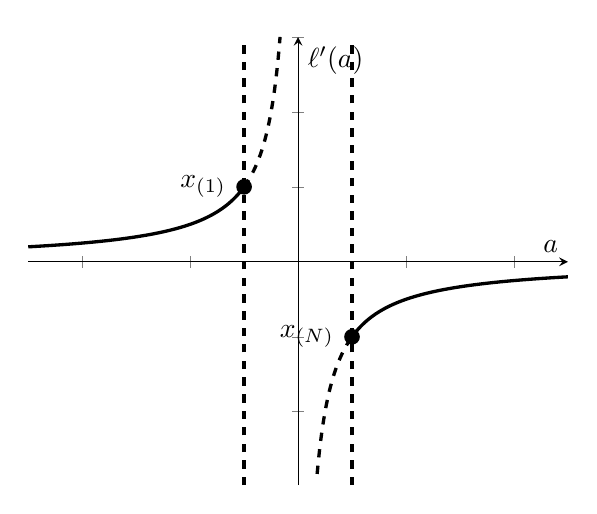
\begin{tikzpicture}
    \begin{axis}[
      samples=100,
      domain=-5:5,
      axis x line=middle,
      axis y line=middle,
      restrict y to domain=-3:3,
      xlabel=$a$,
      ylabel=$\ell'(a)$,
      xticklabels={,,},
      yticklabels={,,}]
      \addplot[
      very thick,
      dashed,
      domain=-1:1
      ] plot(\x, {-1/\x});
      \addplot[
      very thick,
      domain=-5:-1
      ] plot(\x, {-1/\x});
      \addplot[
      very thick,
      domain=1:5
      ] plot(\x, {-1/\x});
      \addplot[
      very thick,
      dashed
      ] plot(-1, \x);
      \addplot[
      very thick,
      dashed
      ] plot(1, \x);
      \node[label={180:{$x_{(1)}$}}, circle, fill, inner sep=2pt] at
      (axis cs:-1,1) {};
      \node[label={180:{$x_{(N)}$}}, circle, fill, inner sep=2pt] at
      (axis cs:1,-1) {};
    \end{axis}
  \end{tikzpicture}
\end{figure}

For $a < 0$, the likelihood is increasing, so it will be maximized
where $a = x_{(1)}$, assuming that $|x_{(1)}| \ge |x_{(N)}|$.
Similarly, for $a > 0$, the likelihood is decreasing, so it is
maximized where $a = x_{(n)}$, assuming that
$|x_{(N)}| \ge |x_{(1)}|$. This function is only defined when
$\max_i |x_i| \le a$. This means that $\ell$ is maximized at
$a = \max( |x_{(1)}|, |x_{(n)}| )$.

\subsection{b.}
$p(x_{n+1}) = \frac{1}{b-a} = \frac{1}{2a}$

\subsection{c.}
Our approach is not Bayesian, so we will assign zero probability to
$x_{n+1} > a$ and $x_{n+1} < -a$. A better solution would be to derive
$\hat{a}_{MAP}$ and give a plug-in approximation.

\section{Bayesian analysis of the uniform distribution}

We must derive the posterior, $p(D|\theta)$ given the following:

\begin{equation}
  p(D,\theta) = \frac{Kb^K}{\theta^{N+K+1}} \mathbb{I}(\theta \ge
  \max(D,b)) \\
\end{equation}

Let $m = \max(D)$.

\begin{align*}
  p(D) &= \int_m^\infty \frac{Kb^K}{\theta^{N+K+1}} \; d\theta \\
       &= \left\{ \begin{array}{ll}
                    \frac{K}{(N+K)b^N} & \mbox{if $m \le b$} \\
                    \frac{Kb^K}{(N+K)m^{N+K}} & \mbox{if $m >
                                                b$} \end{array}
                                                \right. \numberthis \\
\end{align*}

\begin{align*}
  p(\theta|D) &= \frac{p(\theta,D)}{p(D)} \\
              &= \left\{ \begin{array}{ll}
                           \frac{Kb^K}{\theta^{N+K+1}} \cdot
                           \frac{(N+K)b^N}{K} & \mbox {if $m \le b \le
                           \theta$} \\
                           \frac{Kb^K}{\theta^{N+K+1}} \cdot
                           \frac{(N+K)m^{N+K}}{Kb^K} & \mbox {if $b < m
                           \le \theta$} \end{array} \right. \\
              &= \left\{ \begin{array}{ll}
                           (N+K) \cdot b^{N+K} \cdot \theta^{-(N+K+1)} & \mbox {if $m \le b \le
                           \theta$} \\
                           (N+K) \cdot m^{N+K} \cdot \theta^{-(N+K+1)} & \mbox {if $b < m
                           \le \theta$} \end{array} \right. \\
              &\propto \left\{ \begin{array}{ll}
                           \text{Pareto}(\theta|N+K,b)& \mbox {if $m \le b \le
                           \theta$} \\
                           \text{Pareto}(\theta|N+K,m)& \mbox {if $b < m
                           \le \theta$} \end{array} \right. \\
              &= \text{Pareto}(\theta|N+K, \max(m,b))
\end{align*}

\section{Taxicab (tramcar) problem}

\begin{equation}
  \text{Pareto}(\theta|N+K, \max(m,b))  
\end{equation}

\subsection{a.}
Given a non-informative prior, $ \text{Pareto}(\theta|0,0)$:

\begin{align*}
  p(\theta|D) &= \text{Pareto}(\theta|1 + 0, \max(100, 0)) \\
              &= \text{Pareto}(\theta|1, 100)
\end{align*}

\subsection{b.}

$ E[\theta|D] = \frac{km}{k - 1} \text{ and } k = 1$, so the posterior
mean is not defined.

The mode is $\max(D) = 100$.

\begin{align*}
  \int_{100}^x km^k \theta^{-(k+1)} \; d\theta &= \frac{1}{2} \\
  100 \int_{100}^x \theta^{-2} \; d\theta &= \frac{1}{2} \\
  \left[ - \frac{1}{\theta} \right]_{100}^x &= \frac{1}{200} \\
  -  \frac{1}{x} + \frac{1}{100} &= \frac{1}{200} \\
  x &= 200
\end{align*}

The median is 200.

\subsection{c.}

\begin{align*}
  p(D'|D,\alpha) &= \int_\theta p(D'|\theta) p(\theta|D,\alpha) \;
                   d\theta) \\
                 &= \int_\theta \frac{1}{\theta} \mathbb{I}(x \le
                   \theta) \cdot N \cdot m^N \cdot \theta^{-(N+1)} \;
                   d\theta \\
                 &= Nm^N \int_\theta \theta^{-(N+2)} \; d\theta \\
                 &= Nm^N \left[ -\frac{1}{N-1} \theta^{-N-1}
                   \right]_{\max(x,m)}^\infty \\
                 &= Nm^N \left[ 0 - \left( -\frac{1}{N-1}
                   \max(x,m)^{-N-1} \right) \right] \\
                 &= \frac{Nm^N}{(N+1)\max(x,m)^{N+1}} \\
                 &= \left\{ \begin{array}{ll}
                              \frac{N}{m(N+1)} & \mbox{if $x < m$} \\
                              \frac{Nm^N}{x^{N+1}(N+1)} & \mbox{if $x
                                                          \ge m$}
                            \end{array} \right.
\end{align*}

\subsection{d.}

\begin{equation*}
  \begin{split}
    p(x = 100|D,\alpha) &= \frac{1 \cdot 100^1}{(1+1)100^{1+1}} =
    \frac{1}{200} \\
    p(x = 50|D,\alpha) &= \frac{1}{(1+1)100} = \frac{1}{200} \\
    p(x = 150|D,\alpha) &= \frac{1 \cdot 100^1}{(1+1)150^{1+1}} =
    \frac{1}{450}
  \end{split}
\end{equation*}

\subsection{e.}
To improve the accuracy we could use a more informative prior. For
example, we could estimate the number of cabs based on the city's
population. Accuracy will also improve with more observations.

\section{Bayesian analysis of the exponential distribution}

\subsection{a.}

\begin{gather*}
  p(x|\theta) = \theta e^{-\theta x} \quad \text{for } x \ge 0, \theta
  \ge 0 \\
  p(D|\theta) = \prod_{i=1}^N p(x_i|\theta) = \prod_{i=1}^N \theta
  e^{-\theta x_i}
\end{gather*}

\begin{align*}
  \ln (p(D|\theta)) &= \sum_{i=1}^N \ln \theta e^{-\theta x_i} \\
                    &= \sum_{i=1}^N \ln \theta + \ln e^{-\theta x_i}
  \\
                    &= \sum_{i=1}^N \ln \theta + -\theta x_i \\
  \frac{d}{d\theta} (\sum_{i=1}^N \ln \theta + -\theta x_i) &=
                                                              \sum_{i=1}^N
                                                              \frac{1}{\theta}
                                                              - x_i \\
  0 &= \frac{N}{\theta} - \sum_{i=1}^N x_i \\
  \hat{\theta} &= \frac{N}{\sum_{i=1}^N x_i} \\
  \hat{\theta} &= \frac{1}{\frac{1}{N} \sum_{i=1}^N x_i}
\end{align*}

\subsection{b.}
\begin{align*}
  \hat{\theta} &= \frac{1}{\frac{1}{N} \sum_{i=1}^N x_i} \\
               &= \frac{1}{\frac{1}{3}(5+6+4)} \\
               &= \frac{1}{5}
\end{align*}

\subsection{c.}

\begin{align*}
  p(\theta) &= \text{Expon}(\theta|\lambda) \\
            &= \lambda e^{-\lambda \theta} \\
            &= \frac{\lambda^1}{\Gamma(1)} \theta^{1-1} e^{-\lambda \theta} \\
            &= \text{Ga}(\theta|1, \lambda)
\end{align*}

The mean of the Gamma distribution is $\frac{1}{\lambda}$, so
$\hat{\lambda} = 3$

\subsection{d.}

\begin{equation*}
  p(\theta|D,\hat{\lambda}) \propto p(D|\theta) p(\theta|\hat{\lambda}) \\
\end{equation*}

\begin{align*}
    p(D|\theta) &= \prod_{x=1}^N \theta e^{-\theta x_i} \\
                &= \theta e^{-\theta x_1} \cdot \theta e^{-\theta x_2}
                  \cdot \theta e^{-\theta x_3} ... \\
                &= \theta^N e^{(-\theta x_1 -\theta x_2 -\theta x_3
                  ...)} \\
                &= \theta^N e^{-\theta \sum x_i}
\end{align*}

\begin{equation*}
  p(\theta|\hat{\lambda}) = \hat{\lambda} e^{-\theta \hat{\lambda}}
\end{equation*}

\begin{align*}
  p(\theta|D,\hat{\lambda}) &\propto \theta^N e^{-\theta \sum x_i}
  \hat{\lambda} e^{-\theta \hat{\lambda}} \\
  &\propto \theta^N e^{-\theta(\hat{\lambda} + \sum x_i)} \\
  &= \text{Ga}(\theta|N+1, \hat{\lambda} + \sum_{i=1}^N x_i)
\end{align*}

\subsection{e.}

Yes, the prior is equivalent to a Gamma distribution and the posterior
is also a Gamma distribution.

\subsection{f.}

The mean of a Ga$(\theta|a,b)$ distribution is $\frac{a}{b}$. The mean
of \mbox{Ga$(\theta|N+1, \hat{\lambda} + \sum_{i=1}^N x_i)$} $= \frac{N+1}{ \hat{\lambda} + \sum_{i=1}^N x_i}$

\subsection{g.}

The posterior accounts for the exponential prior. The prior accounts
for expert knowledge, thus it is more reasonable.

\section{MAP estimate for the Bernoulli with non-conjugate priors}

\subsection{a.}

We're looking for the MAP estimate for $\theta$, defined as $\hat{\theta}_{MAP} = \underset{\theta}{\mathrm{argmax}} p(\theta|D)$

We can calculate the posterior up to normalization constants given the
number of occurrences of heads and tails and the piecewise function
that defines the prior.

\begin{align*}
  p(\theta|D) &\propto p(D|\theta) \cdot p(\theta) \\
              &= \theta^{N_1}(1 - \theta)^{N_0} \cdot
                \left\{ \begin{array}{ll}
                          .5 & \mbox{if $\theta = .4 \text{ or } .5$} \\
                          0 & \mbox{else} \end{array} \right. \\
              &= \left\{ \begin{array}{ll}
                                 \theta^{N_1}(1 - \theta)^{N - N_1} &
                                                                      \mbox{if
                                                                      $\theta
                                                                      \in
                                                                      \{.4,
                                                                      .5\}$} \\
                                 0 & \mbox{else} \end{array} \right.
  \\
              &= \left\{ \begin{array}{ll}
                           .4^{N_1}(.6)^{N - N_1} & \mbox{if $\theta = .4$} \\
                           .5^N & \mbox{if $\theta = .5$} \\
                           0 & \mbox{else} \end{array} \right.
  \\
\end{align*}
The MAP estimate is the value of $\theta$ that maximizes the equation above.

\begin{equation*}
  \hat{\theta}_{MAP} = \left\{ \begin{array}{ll}
                           .4 & \mbox{if $(.4)^{N_1} (.6)^{N-N_1} \ge .5^N$} \\
                           .5 & \mbox{else} \end{array} \right.
\end{equation*}

\subsection{b.}
If N is small, $\theta = .4$ will lead to a better estimate since the
prior is close to the true value. As N grows, the data will overwhelm
the prior.

\section{Posterior predictive distribution for a batch of data with
the Dirichlet-multinomial model}
\label{3.13}

\begin{align*}
  p(D'|D,\alpha) &= \int_\theta p(D'|\theta) \cdot p(\theta|D) d\theta
  \\
                 &= \int_\theta \text{Mu}(N_{new_1}, N_{new_2},...|\theta) \cdot
                   \text{Dir}(\theta|N_{old_1} + \alpha_1, N_{old_2} + \alpha_2 ...)
  \\
                 &= \frac{1}{\text{B}(\alpha + N_{old})} {N_{new}!
                   \choose N_{new_1}! ... N_{new_k}!} \int_{\theta}
                   \prod^k \theta_k^{N_{new_k}} \cdot \prod^k
                   \theta_k^{\alpha_k + N_{old_k}
                   - 1} \; d\theta \\
                 &= \frac{1}{\text{B}(\alpha + N_{old})} {N_{new}!
                   \choose N_{new_1}! ... N_{new_k}!} \int_{\theta} \underbrace{
                   \prod^k \theta_k^{\alpha_k + N_{new_k} + N_{old_k}
                   - 1} \; d\theta}_{\text{normalization constant for
                   Dir($\vec{\alpha} + \vec{N_{new}} +
                   \vec{N_{old}}$)}} \\
                 &= {N_{new}! \choose N_{new_1}! ... N_{new_k}!}
                   \frac{B(\alpha + N_{old} + N_{new})}{B(\alpha +
                   N_{old})} \\
                 &= \frac{N'_0!}{\prod N'_k!} \cdot \frac{\prod
                   \Gamma(\alpha_k + N_k + N'_k)}{\Gamma(\alpha_0 + N_0
                   + N_0')} \cdot \frac{\Gamma(\alpha_0 + N_0)}{\prod
                   \Gamma(\alpha_k + N_k)} \quad \text{where
                   $\alpha_0 = \sum_{i=1}^k \alpha_i, N_0 = \sum_{i=1}^k
                   N_i, \text{ and } N'_0 = \sum_{i=1}^k N'_i$} \\
                 &= \frac{N'_0!}{\prod N'_k!} \cdot \frac{\Gamma(\alpha_0 +
                   N_0)}{\Gamma(\alpha_0 + N_0 + N'_0)} \cdot
                   \frac{\prod \Gamma(\alpha_k + N_k + N'_k)}{\prod
                   \Gamma(\alpha_k + N_k)}
\end{align*}

Notice that this looks like the formula we derived in exercise
\ref{3.2}.

\section{Posterior predictive for Dirichlet-multinomial}

\subsection{a.}

\begin{align*}
  p(X=j|D) &= E[\theta_j|D] \qquad \text{Equation (3.51) in the
  textbook} \\
           &= \frac{\alpha_j + N_j}{\alpha_0 + N} \\
           &= \frac{10 + 260}{(10 \cdot 27) + 2000} \\
           &= .119
\end{align*}

\subsection{b.}

We use the equation from \ref{3.13}.

\begin{equation*}
  p(D'|D,\alpha) = \frac{N'_0!}{\prod N'_k!} \cdot \frac{\Gamma(\alpha_0 +
                   N_0)}{\Gamma(\alpha_0 + N_0 + N'_0)} \cdot
                   \frac{\prod \Gamma(\alpha_k + N_k + N'_k)}{\prod
                   \Gamma(\alpha_k + N_k)}
\end{equation*}

For a single trial, $ N'_0 = N'_j= 1$, so the first term is equal to
1. Now we examine the last term.

\begin{align*}
  p(x=j|D,\alpha) &= \frac{\Gamma(\alpha_0 + N_0)}{\Gamma(\alpha_0 + N_0 + N'_0)}
             \cdot \frac{\prod_{k \neq j} \Gamma(\alpha_k + N_k +
             N'_k)}{\prod_{k \neq j} \Gamma(\alpha_k + N_k)} \cdot
             \frac{\Gamma(\alpha_j + N_j + N'_j)}{\Gamma(\alpha_j +
             N_j)} \\
           &= \frac{\Gamma(\alpha_0 + N_0)}{\Gamma(\alpha_0 + N_0 + N'_0)}
             \cdot \prod_{k \neq j} \frac{\Gamma(\alpha_k + N_k +
             0)}{\Gamma(\alpha_k + N_k)} \cdot \frac{\Gamma(\alpha_j +
             N_j + N'_j)}{\Gamma(\alpha_j + N_j)} \\
           &= \frac{\Gamma(\alpha_0 + N_0)}{\Gamma(\alpha_0 + N_0 + N'_0)}
             \cdot 1 \cdot \frac{\Gamma(\alpha_j +
             N_j + N'_j)}{\Gamma(\alpha_j + N_j)} \\
           &= \frac{\Gamma(\alpha_0 + N_0)}{\Gamma(\alpha_0 + N_0 + 1)}
             \cdot \frac{\Gamma(\alpha_j +
             N_j + 1)}{\Gamma(\alpha_j + N_j)} \\
           &= \frac{\Gamma(\alpha_0 + N_0)}{(\alpha_0 +
             N_0)\Gamma(\alpha_0 + N_0)} \cdot \frac{(\alpha_j +
             N_j)\Gamma(\alpha_j + N_j)}{\Gamma(\alpha_j + N_j)} \\
           &= \frac{\alpha_j + N_j}{\alpha_0 + N_0}
\end{align*}

For independent samples

\begin{align*}
  p(x_{2001}=a, x_{2002}=p|D,\alpha) &= p(x_{2001}=a|D,\alpha)
                                           \cdot
                                           p(x_{2002}=p|D',\alpha)
  \\
                                         &= \frac{10 + 100}{270 +
                                           2000} \cdot \frac{10 +
                                           87}{270 + 2001} \\
                                         &= .0021
\end{align*}

\end{document}
